\documentclass[11pt,a4paper]{ivoa}
\input tthdefs

\title{IVOA DataLink}

% see ivoatexDoc for what group names to use here
\ivoagroup{DAL}

\author[http://www.ivoa.net/twiki/bin/view/IVOA/PatrickDowler]
       {Patrick Dowler}
\author[http://www.ivoa.net/twiki/bin/view/IVOA/FrancoisBonnarel]
       {Fran\c{c}ois Bonnarel}
\author[http://www.ivoa.net/twiki/bin/view/IVOA/LaurentMichel]
       {Laurent Michel}
\author[http://www.ivoa.net/twiki/bin/view/IVOA/MarkusDemleitner]
       {Markus Demleitner}
\editor[http://www.ivoa.net/twiki/bin/view/IVOA/PatrickDowler]
       {Patrick Dowler}

% \previousversion[????URL????]{????Concise Document Label????}
\previousversion{This is the first public release}
       

\begin{document}

\begin{abstract}
This document describes the linking of data discovery metadata
to access to the data itself, further detailed metadata, related
resources, and to services that perform operations on the data. The web
service capability supports a drill-down into the details of a specific
dataset and provides a set of links to the dataset file(s) and related
resources. This specification also includes a VOTable-specific method
of providing descriptions of one or more services and their input(s),
usually using parameter values from elsewhere in the VOTable document.
Providers are able to describe services that are relevant to the records
(usually datasets with identifiers) by including service descriptors in
a result document.
\end{abstract}


\section*{Acknowledgments}

The authors would like to thank all the participants in DAL-WG discussions
for their ideas, critical reviews, and contributions to this document.


\section*{Conformance-related definitions}

The words ``MUST'', ``SHALL'', ``SHOULD'', ``MAY'', ``RECOMMENDED'', and
``OPTIONAL'' (in upper or lower case) used in this document are to be
interpreted as described in IETF standard RFC2119 \citep{std:RFC2119}.

The \emph{Virtual Observatory (VO)} is a
general term for a collection of federated resources that can be used
to conduct astronomical research, education, and outreach.
The \href{http://www.ivoa.net}{International
Virtual Observatory Alliance (IVOA)} is a global
collaboration of separately funded projects to develop standards and
infrastructure that enable VO applications.


\section{Introduction}

???? Write something ????

\subsection{Role within the VO Architecture}

\begin{figure}
\centering

% As of ivoatex 1.2, the architecture diagram is generated by ivoatex in
% SVG; copy ivoatex/archdiag-full.xml to archdiag.xml and throw out
% all lines not relevant to your standard.
% Notes don't generally need this.  If you don't copy archdiag.xml,
% you must remove archdiag.svg from FIGURES in the Makefile.

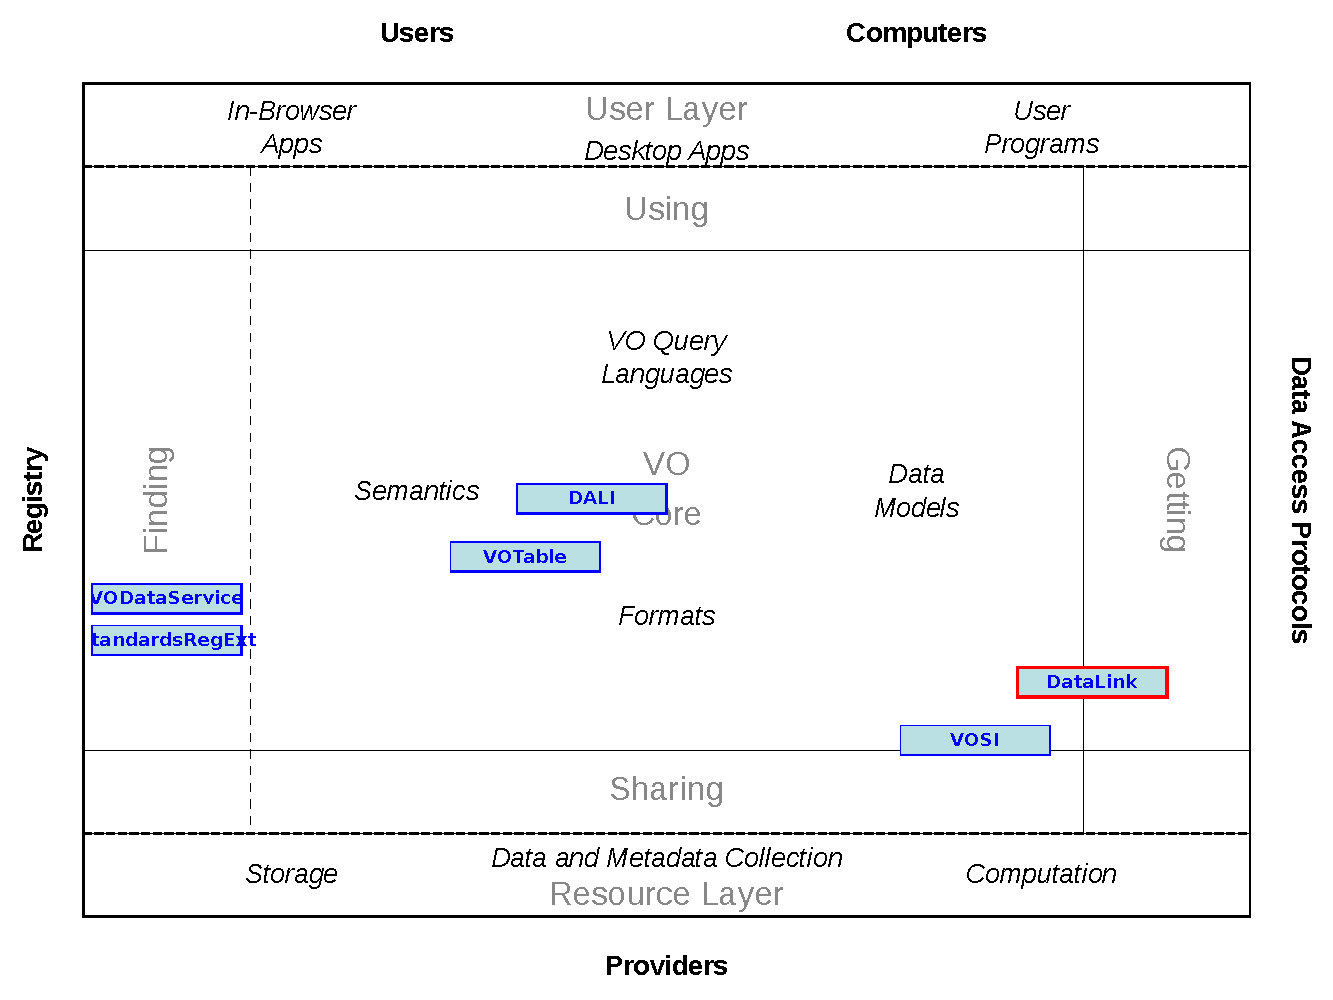
\includegraphics[width=0.9\textwidth]{role_diagram.pdf}
\caption{Architecture diagram for this document}
\label{fig:archdiag}
\end{figure}

Fig.~\ref{fig:archdiag} shows the role this document plays within the
IVOA architecture \citep{note:VOARCH}.

???? and so on, LaTeX as you know and love it. ????

\appendix
\section{Changes from Previous Versions}

No previous versions yet.  
% these would be subsections "Changes from v. WD-..."
% Use itemize environments.


% NOTE: IVOA recommendations must be cited from docrepo rather than ivoabib
% (REC entries there are for legacy documents only)
\bibliography{ivoatex/ivoabib,ivoatex/docrepo}


\end{document}
